\documentclass[12pt,aspectratio=169]{beamer}


\usepackage{algorithm,algorithmic}

\usepackage[utf8]{inputenc}
\usepackage{booktabs}
\usepackage[opacity=0.1]{pdfcomment} % set to 0 to make annotation icons invisible
\usepackage{pdfpc}
\usepackage{arev}
\usepackage{multicol}

\usepackage{xcolor, color, colortbl}
\definecolor{dkgreen}{rgb}{0,0.5,0}
\definecolor{dkred}{rgb}{0.8,0,0}
\definecolor{dkblue}{rgb}{0,0,0.5}
\definecolor{gray}{rgb}{0.5,0.5,0.5}
\definecolor{mauve}{rgb}{0.58,0,0.82}
\definecolor{hilight}{RGB}{122,86,0}

\definecolor{LRed}{rgb}{1,.8,.8}
\definecolor{MRed}{rgb}{1,.6,.6}
\definecolor{HRed}{rgb}{1,.2,.2}

\usepackage{tikz}
\usetikzlibrary{arrows.meta,
                calc, chains,
                quotes,
                positioning,
                shapes.geometric}


\def\scalefact{0.85}
\newcommand{\cev}[1]{\reflectbox{\ensuremath{\vec{\reflectbox{\ensuremath{#1}}}}}}
\newcommand{\evalat}[2]{\left.#1\right\vert_{#2}}

\newcommand{\znode}[5][black]{\path (#3,#4) node(#2) [circle,draw,color=#1] {#5};}
\newcommand{\zunedge}[6][black]{%
\begin{scope}
	\path (#2,#3) node(this) [inner sep=0pt,triangle,draw,color=#1] {#4};
	\draw[->,color=#1] (#5) -- (this.west);
	\draw[->,color=#1] (this.east) -- (#6);
\end{scope}}
\newcommand{\zbiedge}[7][black]{%
\begin{scope}
	\path (#2,#3) node(this) [inner sep=0pt,triangle,draw,color=#1] {#4};
	\draw[->,color=#1] (#5) -- (this);
	\draw[->,color=#1] (#6) -- (this);
	\draw[->,color=#1] (this.east) -- (#7);
\end{scope}}
\newcommand{\zedge}[5][black]{\path (#3,#4) node(#2) [inner sep=0pt,triangle,draw,color=#1] {#5};}

\definecolor{blue(pigment)}{rgb}{0.2, 0.2, 0.6}
\definecolor{burgundy}{rgb}{0.5, 0.0, 0.13}


\usepackage{listings}
%% \usetheme{Goettingen}
\usefonttheme{serif}
\usepackage{times}
\setbeamertemplate{navigation symbols}{}

\title{Deep Learning}
\subtitle{Lecture 6: Gradient Descent}
 
 
%\author[Mehrdad Maleki] % (optional, for multiple authors)
%{Mehrdad Maleki, Barak A. Pearlmutter\footnote{ Institute & Department of Computer Science
%Maynooth University, Co. Kildare, Ireland}, Jeffrey Mark Siskind}
 
%\institute[NUIM] % (optional)
%{
%  Department of Computer Science \\
%  National University of Ireland Maynooth
 
%}

\author[]{\textbf{Dr. Mehrdad Maleki}}
%\institute[]{\textsuperscript{1}Department of Computer Science\\ National University of Ireland\\ Maynooth}
% 
\date{}
 
%\logo{\includegraphics[height=1.5cm]{lion-logo.png}}

\renewcommand{\Re}{\mathbb{R}}
 
\begin{document}
 
\frame{\titlepage}

%\begin{frame}
%\frametitle{Motivation}
%Suppose you need to predict the next move of your component in the chess based on the previous move. If you write down all the possible moves from the current move they are tremendously large combinations. So minimizing the error is not feasible. Instead you can record sample of the same move in previous moves and use that for the error function.
%\end{frame}

\begin{frame}
\frametitle{Motivation}
You have a NN that meant to compute desire function $g(\mathbf{X})$. But your NN actually compute $f(\mathbf{X},\mathbf{W})$ and you need to find the value of $\mathbf{W}$ such that $\|g(\mathbf{X})-f(\mathbf{X},\mathbf{W})\|$ is minimum. But the value of $g(\mathbf{X})$ is not known for all $\mathbf{X}$. So we sample the function $g$. On input $\mathbf{X_i}$ if $\mathbf{y_i}=g(\mathbf{X_i})$ then for $i=1,\dots ,N$, $\{(\mathbf{X_i},\mathbf{y_i}):1\leq i\leq N\}$ is the set of samples.

\end{frame}

\begin{frame}
\begin{figure}
\begin{tikzpicture}
\draw[ultra thick,->] (0,0) -- (5,0);
\draw[ultra thick,->] (0,0) -- (0,5);
\node[below] at (5,0) {$x_1$};
\node[left] at (0,5) {$x_2$};\pause
\fill[red] (2,3) circle [radius=4pt];\pause
\fill[red] (2,4) circle [radius=4pt];\pause
\fill[blue] (1,-1) circle [radius=4pt];\pause
\fill[red] (0,1) circle [radius=4pt];\pause
\fill[blue] (3,0) circle [radius=4pt];\pause
\fill[red] (3.5,4) circle [radius=4pt];\pause
\fill[red] (-1,3) circle [radius=4pt];\pause
\fill[blue] (4,3) circle [radius=4pt];\pause
\fill[blue] (1,0.7) circle [radius=4pt];\pause
\fill[red] (-3,3) circle [radius=4pt];\pause
\draw[fill=pink,draw=none,rotate around={-45:(-1,-1)}] (-1,-1) rectangle (-6,6);
\fill[red] (2,3) circle [radius=4pt];
\fill[red] (2,4) circle [radius=4pt];
\fill[blue] (1,-1) circle [radius=4pt];
\fill[red] (0,1) circle [radius=4pt];
\fill[blue] (3,0) circle [radius=4pt];
\fill[red] (3.5,4) circle [radius=4pt];
\fill[red] (-1,3) circle [radius=4pt];
\fill[blue] (4,3) circle [radius=4pt];
\fill[blue] (1,0.7) circle [radius=4pt];
\fill[red] (-3,3) circle [radius=4pt];
\draw[thick, green] (-1.2,-1.2) -- (5,5);
\draw[ultra thick,->] (0,0) -- (5,0);
\draw[ultra thick,->] (0,0) -- (0,5);

\node[below] at (5,0) {$x_1$};
\node[left] at (0,5) {$x_2$};
\end{tikzpicture}
\end{figure}
\end{frame}

\begin{frame}
\begin{figure}
\begin{tikzpicture}
\draw[thick,->] (0,1) -- (2,0.1);
\node[left] at (0,1) {$x_1$}; 
\draw[thick,->] (0,-1) -- (2,-0.1);
\node[left] at (0,-1) {$x_2$};\pause
\node[above,orange] at (1,0.5) {$w_1$};\pause
\node[below,orange] at (1,-0.5) {$w_2$};\pause
\draw[thick] (2.5,0) circle (15pt);\pause
\node[ultra thick, blue] at (2.5,0) {$+$};\pause
\draw[thick,->] (3,0) -- (4,0);\pause
\draw[] (4,-0.5) rectangle (5,0.5);
\draw[ultra thick, green] (4,-0.1) -- (4.5,-0.1);
\draw[ultra thick, green] (4.5,-0.1) -- (4.5,0.3);
\draw[ultra thick, green] (4.5,0.3) -- (5,0.3);\pause
\draw[thick,->] (5,0) -- (6,0);\pause
\node[right,brown] at (6,0) {$ y = \left\{ \begin{array}{ll}
        1 & \mbox{if $w_1x_1+w_2x_2 \geq 0$}\\ \pause
        0 & \mbox{else} \end{array} \right. $ };
\end{tikzpicture}
\end{figure}
\end{frame}

\begin{frame}


We know that,
\[
\begin{tabular}{|c|c|c|c|}
\hline
 & \textcolor{red}{Red} &  & \textcolor{blue}{Blue} \\
\hline
1 & $g(2,3)= 1$ & 7 & $g(1,-1)=0$\\
2 & $g(2,4)=1$ & 8 & $g(3,0)=0$\\
3 & $g(0,1)=1$ & 9 & $g(4,3)=0$\\
4 & $g(3.5,4)=1$ & 10 & $g(1,0.7)=0$\\
5 & $g(-1,3)=1$ & &\\
6 & $g(-3,3)=1$ &  &\\
\hline
\end{tabular}
\]
we need to find the parameters $w_1, w_2$ such that if 
\[
 f(x_1,x_2\,;w_1,w_2) = \left\{ \begin{array}{ll}
        1 & \mbox{if $w_1x_1+w_2x_2 \geq 0$}\\ 
        0 & \mbox{else} \end{array} \right. \]
then,
\[
\sum_{i=1}^{10} \|f(x_1^{(i)},x_2^{(i)})\,;w_1,w_2)-g(x_1^{(i)},x_2^{(i)})\|
\]
is minimum.
\end{frame}

\begin{frame}
Suppose we only have one point with red label, i.e., 1. Then the optimal weight vector for this point is as follow, \pause
\begin{figure}
\begin{tikzpicture}
\draw[->] (0,0) -- (5,0);
\node[below] at (5,0) {$x_1$};
\draw[->] (0,0) -- (0,5);
\node[left] at (0,5) {$x_2$};
\fill[red] (2,4) circle [radius=4pt];\pause
\draw[thick, blue,->] (0,0) -- (2,4);\pause
\node[above] at (2,4) {$\mathbf{W}=\begin{bmatrix}
w_1\\
w_2
\end{bmatrix}$};\pause
\draw[ultra thick,green] (-2,1) -- (2,-1);
\draw[fill=pink,draw=none,rotate around={-26.5:(0,0)}] (-2,0) rectangle (2,5);
\draw[->] (0,0) -- (5,0);
\node[below] at (5,0) {$x_1$};
\draw[->] (0,0) -- (0,5);
\node[left] at (0,5) {$x_2$};
\fill[red] (2,4) circle [radius=4pt];
\draw[thick, blue,->] (0,0) -- (2,4);
\node[above] at (2,4) {$\mathbf{W}=\begin{bmatrix}
w_1\\
w_2
\end{bmatrix}$};
\end{tikzpicture}
\end{figure}
\end{frame}


\begin{frame}
Suppose we only have one point with blue label, i.e., -1. Then the optimal weight vector for this point is as follow, \pause
\begin{figure}
\begin{tikzpicture}
\draw[->] (0,0) -- (5,0);
\node[below] at (5,0) {$x_1$};
\draw[->] (0,0) -- (0,5);
\node[left] at (0,5) {$x_2$};
\fill[blue] (1,-1) circle [radius=4pt];\pause
\draw[thick, blue,->] (0,0) -- (-1,1);\pause
\node[above] at (-1,1) {$\mathbf{W}=\begin{bmatrix}
w_1\\
w_2
\end{bmatrix}$};\pause
\draw[ultra thick,green] (-1,-1) -- (2,2);
\draw[fill=pink,draw=none,rotate around={45:(0,0)}] (-2,0) rectangle (2,5);
\draw[->] (0,0) -- (5,0);
\node[below] at (5,0) {$x_1$};
\draw[->] (0,0) -- (0,5);
\node[left] at (0,5) {$x_2$};
\fill[blue] (1,-1) circle [radius=4pt];
\draw[thick, blue,->] (0,0) -- (-1,1);
\node[above] at (-1,1) {$\mathbf{W}=\begin{bmatrix}
w_1\\
w_2
\end{bmatrix}$};
\end{tikzpicture}
\end{figure}
\end{frame}


\begin{frame}
\begin{figure}
\begin{tikzpicture}
\draw[ultra thick,->] (0,0) -- (5,0);
\draw[ultra thick,->] (0,0) -- (0,5);
\node[below] at (5,0) {$x_1$};
\node[left] at (0,5) {$x_2$};
\fill[red] (2,3) circle [radius=4pt];
\fill[red] (2,4) circle [radius=4pt];
\fill[blue] (1,-1) circle [radius=4pt];
\fill[red] (0,1) circle [radius=4pt];
\fill[blue] (3,0) circle [radius=4pt];
\fill[red] (3.5,4) circle [radius=4pt];
\fill[red] (-1,3) circle [radius=4pt];
\fill[blue] (4,3) circle [radius=4pt];
\fill[blue] (1,0.7) circle [radius=4pt];
\fill[red] (-3,3) circle [radius=4pt];
%\draw[fill=pink,draw=none,rotate around={-45:(-1,-1)}] (-1,-1) rectangle (-6,6);
\draw[green] (-3,2) -- (3,-2);
\draw[ultra thick,brown,->] (0,0) -- (1,6/4);
\node[above] at (1,6/4) {$\mathbf{W}_0$};\pause
\draw[dotted, thick] (1,0.7) --(-1,-0.7);\pause
\draw[ultra thick, brown, ->] (0,0) -- (-1,-0.7);\pause
\node[below] at (-1,-0.7) {\textbf{error}};\pause
\draw[ultra thick, brown,->] (1,6/4) -- (0,6/4-0.7);\pause
\draw[ultra thick, brown,->] (0,0) -- (0,6/4-0.7);\pause
\draw[ultra thick, green] (-3,0) -- (6,0);
\node[left] at (0,6/4-0.7) {$\mathbf{W}_1$};
\end{tikzpicture}
\end{figure}
\end{frame}


\begin{frame}
\begin{figure}
\begin{tikzpicture}
\draw[ultra thick,->] (0,0) -- (5,0);
\draw[ultra thick,->] (0,0) -- (0,5);
\node[below] at (5,0) {$x_1$};
\node[left] at (0,5) {$x_2$};
\fill[red] (2,3) circle [radius=4pt];
\fill[red] (2,4) circle [radius=4pt];
\fill[blue] (1,-1) circle [radius=4pt];
\fill[red] (0,1) circle [radius=4pt];
\fill[blue] (3,0) circle [radius=4pt];
\fill[red] (3.5,4) circle [radius=4pt];
\fill[red] (-1,3) circle [radius=4pt];
\fill[blue] (4,3) circle [radius=4pt];
\fill[blue] (1,0.7) circle [radius=4pt];
\fill[red] (-3,3) circle [radius=4pt];
%\draw[fill=pink,draw=none,rotate around={-45:(-1,-1)}] (-1,-1) rectangle (-6,6);
%\draw[green] (-3,2) -- (3,-2);
%\draw[ultra thick,brown,->] (0,0) -- (1,6/4);
%\node[above] at (1,6/4) {$\mathbf{W}_0$};\pause
%\draw[dotted, thick] (1,0.7) --(-1,-0.7);\pause
%\draw[ultra thick, brown, ->] (0,0) -- (-1,-0.7);\pause
%\node[below] at (-1,-0.7) {\textbf{error}};\pause
%\draw[ultra thick, brown,->] (1,6/4) -- (0,6/4-0.7);\pause
\draw[ultra thick, brown,->] (0,0) -- (0,6/4-0.7);\pause
\draw[ultra thick, green] (-3,0) -- (6,0);
\node[left] at (0,6/4-0.7) {$\mathbf{W}_1$};\pause
\draw[dotted, thick] (1,0.7) --(-1,-0.7);\pause
\draw[ultra thick, brown, ->] (0,0) -- (-1,-0.7);\pause
\node[below] at (-1,-0.7) {\textbf{error}};\pause
\draw[ultra thick, brown, ->] (0,6/4-0.7) -- (-1,6/4-1.4);\pause
\draw[ultra thick, brown, ->] (0,0) -- (-1,6/4-1.4);\pause
\node[left] at (-1,6/4-1.4) {$\mathbf{W}_2$};\pause
\draw[ultra thick, green] (-0.1,-1) -- (0.5,5); 
\end{tikzpicture}
\end{figure}
\end{frame}



\begin{frame}
\begin{figure}
\begin{tikzpicture}
\draw[thick,->] (0,1) -- (2,0.1);
\node[left] at (0,1) {$x_1$}; 
\draw[thick,->] (0,-1) -- (2,-0.1);
\node[left] at (0,-1) {$x_2$};\pause
\node[above,orange] at (1,0.5) {$w_1$};\pause
\node[below,orange] at (1,-0.5) {$w_2$};\pause
\draw[thick] (2.5,0) circle (15pt);\pause
\node[ultra thick, blue] at (2.5,0) {$+$};\pause
\draw[thick,->] (3,0) -- (4,0);\pause
\draw[] (4,-0.5) rectangle (5,0.5);
\draw [red,thick] plot [smooth,samples=200, tension=1] coordinates { 
   (4,-0.16) (4.3,-0.1) (4.7,0.3) (5,0.37)};
\draw[thick,->] (5,0) -- (6,0);\pause
\node[right,brown] at (6,0) {$ y = \sigma(w_1x_1+w_2x_2)$ };
\end{tikzpicture}
\end{figure}
\end{frame}

\begin{frame}
$y$ is the probability that the output labe is equal to $1$ if $x_1$ and $x_2$ are given,
\[
\sigma(w_1x_1^{(i)}+w_2x_2^{(i)})=P(label=1|x_1^{(i)},x_2^{(i)})
\]
because,
\[
\begin{aligned}
& w_1x_1^{(i)}+w_2x_2^{(i)}\geq 0\Rightarrow \sigma(w_1x_1^{(i)}+w_2x_2^{(i)})\geq \frac{1}{2}\\
& w_1x_1^{(i)}+w_2x_2^{(i)}< 0\Rightarrow \sigma(w_1x_1^{(i)}+w_2x_2^{(i)})< \frac{1}{2}
\end{aligned}
\]

\end{frame}

\begin{frame}
So the pmf of the output $\hat{y}^{(i)}$ where $\hat{y}^{(i)}\in \{0,1\}$ is the Bernoulli distribution, i.e.,
\[
P(output=\hat{y}^{(i)}|x_1^{(i)},x_2^{(i)})=\sigma(z^{(i)})^{\hat{y}^{(i)}}(1-\sigma(z^{(i)})^{1-\hat{y}^{(i)}}
\]
where $z^{(i)}=w_1x_1^{(i)}+w_2x_2^{(i)}$. So we need to solve the optimization problem,
\[
\max_{w_1,w_2}\,P(output=\hat{y}^{(i)}|x_1^{(i)},x_2^{(i)})
\]
but instead we could solve the following minimization problem,
\[
\min_{w_1,w_2}\,-\hat{y}^{(i)}\log(\sigma(z^{(i)}))-(1-\hat{y}^{(i)})\log(1-\sigma(z^{(i)}))
\]

\end{frame}

\begin{frame}
If we get average over all sample points we have definition of the \textbf{loss function}, i.e. ,
\[
\mathcal{L}(w_1,w_2)=\frac{1}{N}\sum_{i=1}^N-\hat{y}^{(i)}\log(\sigma(z^{(i)}))-(1-\hat{y}^{(i)})\log(1-\sigma(z^{(i)}))
\]
So the goal of the learing is to solve the following minimization problem,
\[
\min_{w_1,w_2}\,\mathcal{L}(w_1,w_2)
\]
\end{frame}

\begin{frame}
\frametitle{Gradient Descent}
To solve unconstraint optimization problem like,
\[
\min_{x_1,x_2}f(x_1,x_2)
\]
we make a guss $(x_1^0,x_2^0)$ that minimize the function $f$ and we start improving this guess by moving in a direction that have a smaller value than $f(x_1^0,x_2^0)$. But this direction is in the opposite of the gradient at $(x_1^0,x_2^0)$. So the next step is,
\[
(x_1^1,x_2^1)=(x_1^0,x_2^0)-\alpha\mathbf{J}_f(x_1^0,x_2^0)
\]
where $\alpha$ is the \textbf{learning rate}.
\end{frame}

\begin{frame}
\frametitle{Gradient Descent}
\begin{enumerate}
\item Make a guess: $(x_1^0,x_2^0)$
\smallskip
\item $n=0$
\smallskip
\item Update: $(x_1^{n+1},x_2^{n+1})=(x_1^{n},x_2^{n})-\alpha\mathbf{J}_f(x_1^{n},x_2^{n})$
\smallskip
\item $n=n+1$
\smallskip
\item If $\|(x_1^{n+1},x_2^{n+1})-(x_1^{n},x_2^{n})\|<\epsilon$ stop otherwise go to 3.

\end{enumerate}
\end{frame}

\begin{frame}
\begin{figure}
\centering
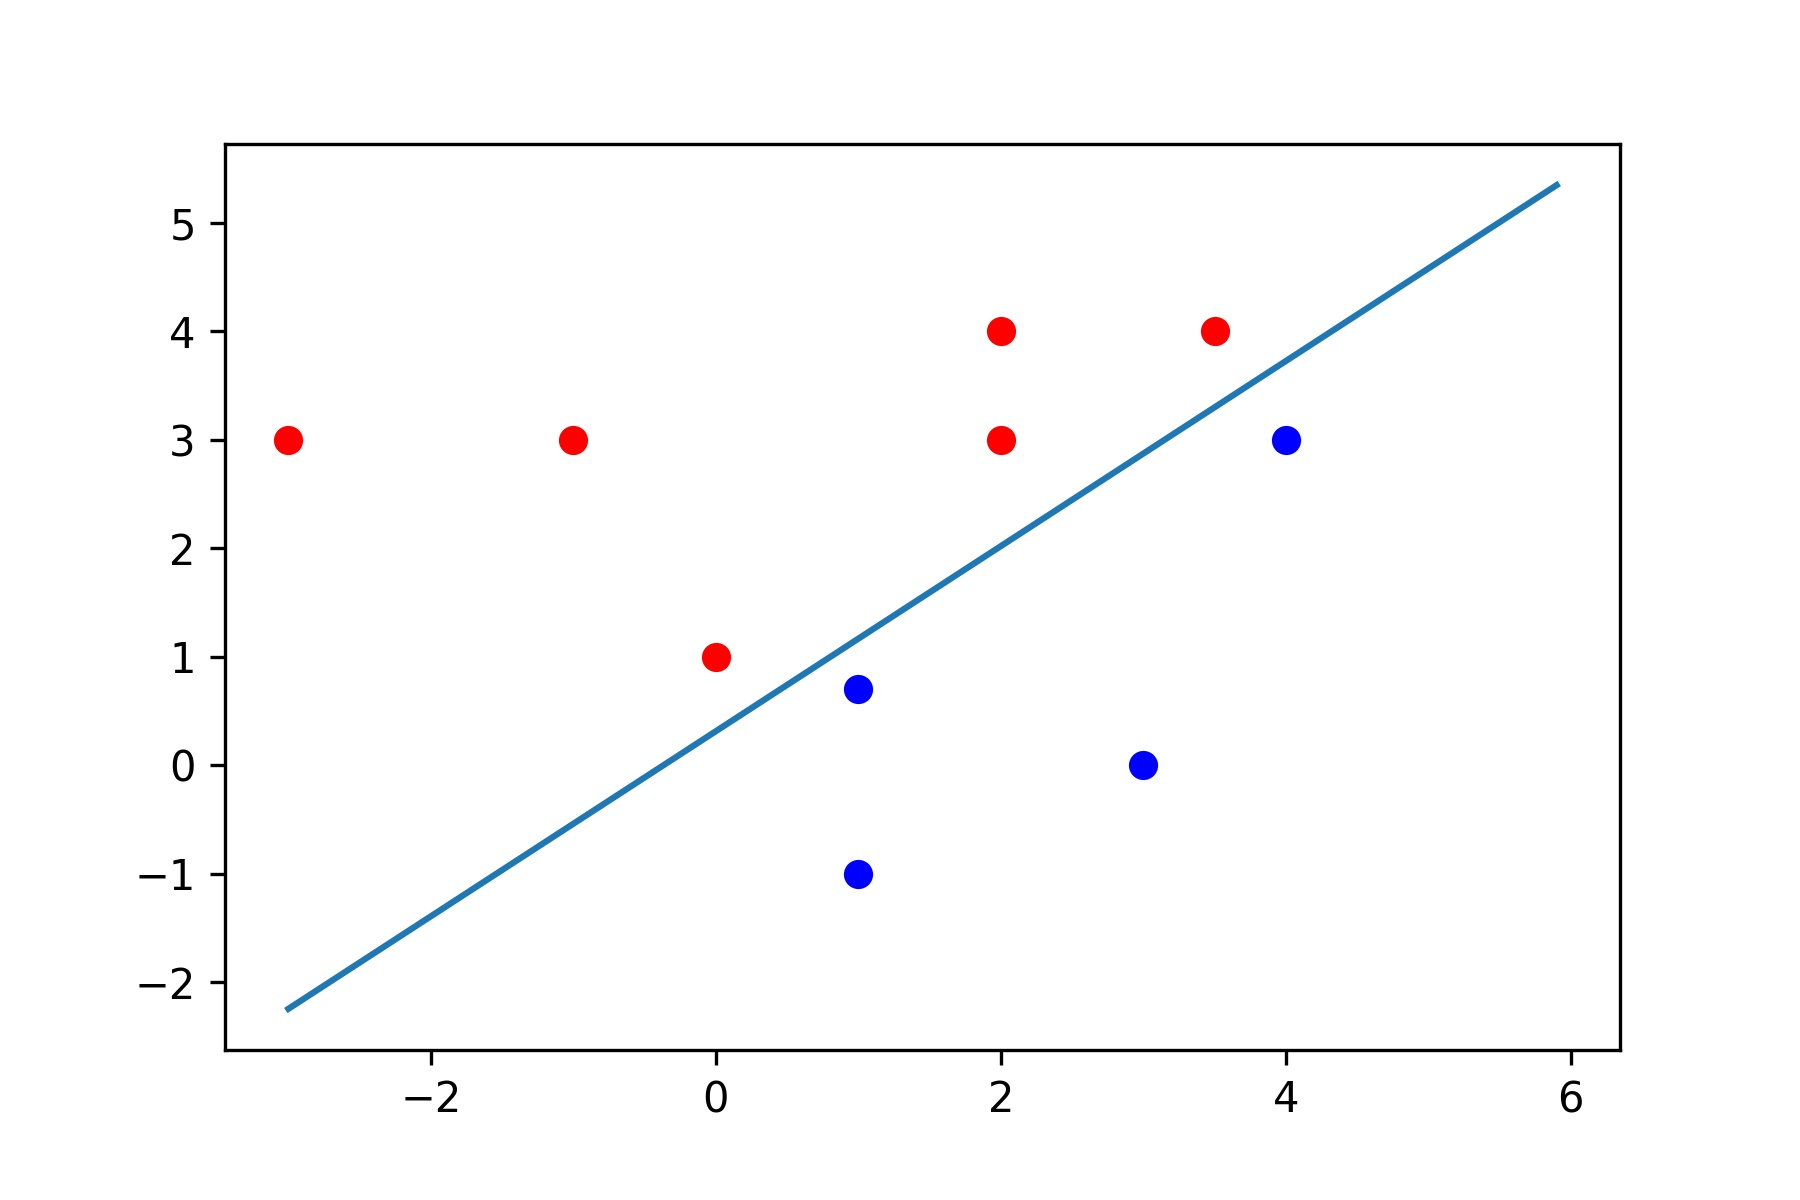
\includegraphics[scale=0.7]{GradDesc}
\caption{Gradient descent for Red/Blue example with 50000 iteration and learning rate $\alpha=0.001$}
\end{figure}
\end{frame}

\begin{frame}{}
  \centering \Huge
  \emph{Thank You}
\end{frame}

\end{document}

